\chapter{Timer/Counters}
\label{cha:timercounters}
In veel applicaties moet even gewacht worden zodat bijvoorbeeld elke minuut een
meting kan worden gedaan.
% Soms moet er een bepaalde tijd worden afgemeten,
%bijvoorbeeld om een waterklep één seconde open te houden.
 Het meten van deze
tijd (wachten) is op te lossen door middel van de bekende wachtlus (zie paragraaf~%
\textbf{??}). De processor kan dan echter geen andere taken
uitvoeren en dat is in veel situaties wél gewenst. Denk hierbij aan Real Time
systemen en besturingssystemen. Beter is deze tijd hardwarematig te meten.
Een \textsl{timer} kan dan uitkomst bieden. Een timer is niets anders dan een teller
die op iedere klokpuls, bijvoorbeeld van de systeemklok, wordt verhoogd. Na een bepaald
aantal klokpulsen heeft de timer de hoogste stand bereikt en begint weer opnieuw.
Er wordt dan een signaal aan de processor afgegeven. Dit signaal genereert, indien geactiveerd, een interrupt, waardoor de processor zijn hoofdprogramma verlaat en een
Interrupt Service Routine gaat uitvoeren.

Dezelfde schakeling kan ook gebruikt worden om extern aangeboden pulsen te tellen.
Denk hierbij aan het tellen van het aantal fietsen dat over een fietspad rijdt.
We noemen zo'n teller een \textsl{counter}. Technisch gezien is er geen verschil
tussen de hardware van een timer en een counter. Het verschil is dus alleen wat
de klokbron is.

De ATmega32 heeft drie timer/counters: een 8-bits Timer/Counter 0 (T/C0), een
16-bits Timer/Counter 1 (T/C1) en een 8 bits Timer/Counter 2 (T/C2).
T/C0 en T/C1 hebben gemeen dat
ze kunnen worden geklokt op een intern kloksignaal en op externe pulsen.
T/C2 kan worden geklokt op een intern kloksignaal en een externe oscillator.
Alle timer/counters hebben diverse interrupt-mogelijkheden en zogenoemde
pulsbreedte gemoduleerde signalen genereren (PWM-signalen). Het is goed om
te weten dat de alle timers min of meer dezelfde mogelijkheden hebben.

In dit hoofdstuk behandelen we de drie timer/counters. Van elke timer/counter
worden de instelmogelijkheden behandeld, zoals de werkmodi, interruptgeneratie
en signaalvormgeneratie. We laten de mogelijkheden zien aan de hand van een aantal
programmavoorbeelden, zowel in assembler als C.

%% Met de combinatie van een counter en een
%%timer kan een \textsl{frequentiemeter} gemaakt worden. E\'en timer meet de tijd van 1
%%seconde en een (andere) counter telt in die tijd het aantal aangeboden pulsen.

\section{Timer/Counter 0}

Timer/Counter 0 is de eerste van de drie timer/counters van de ATmega32 die
besproken worden. Het is een 8-bits timer/counter wat inhoudt dat het kan tellen
tussen 0 en~255. Als de timer/counter intern opgewekte klokpulsen telt spreken
we van een timer. Bij het tellen van extern opgewekte klokpulsen spreken
we van een counter.

Timer/Counter 0 heeft vier werkmodi:

\begin{itemize}
\item Normal mode: Timer/Counter 0 telt van 0 tot en met 255 en begint dan
weer bij 0. Zowel interne ale externe klokpulsen kunnen geteld worden. Deze
modus wordt besproken in paragraaf~\ref{sec:tc0normalmode}.

\item CTC mode: Timer/Counter telt van 0 tot een van te voren opgegeven
maximale waarde en begint dan weer op 0. Zowel interne als externe klokpulsen
kunnen geteld worden. Deze modus wordt besproken in
paragraaf~\ref{sec:tc0ctcmode}.

\item Fast PWM mode: Timer/Counter telt van 0 tot 255 en begint dan weer op~0.
Deze modus wordt voornamelijk gebruikt om een signaalvorm op \'e\'en van de externe
pinnen van de ATmega32 te genereren. Deze modus wordt besproken in
paragraaf~\ref{sec:tc0fastpwmmode}.

\item Phase correct PWM mode: Timer/Counter telt omhoog van 0 tot en met 255
en telt dan weer omlaag tot en met 0. Deze modus wordt voornamelijk gebruikt om een
signaalvorm op \'e\'en van de externe pinnen van de ATmega32 te genereren.
Deze modus wordt besproken in paragraaf~\ref{sec:tc0phasecorrectpwmmode}.
\end{itemize}

In alle werkmodi is het mogelijk om interrupts te genereren. Elke interrupt
is gekoppeld aan een eigen interruptvector.

Bij het programmeren van Timer/Counter 0 worden diverse I/O-registers
gebruikt. Ten eerste is er de Timer/Counter Register (TCNT0). Hierin is de
huidige telwaarde opgeslagen. Ten tweede is er het Output Compare
Register (OCR0). Dit register wordt gebruikt bij de CTC-modus en de beide
PWM-modi. Om T/C0 van de juiste instellingen te voorzien, is er het
Timer/Counter Control Register (TCCR0). Hiermee stellen we onder andere de
werkmodus in.

De vier werkmodi kunnen worden ingesteld met de WGM01- en WGM00-bits in het
TCCR0-register. WGM staat voor \textsl{Waveform Generation Mode}.
De indeling van deze twee bits is te zien in
figuur~\ref{fig:timtccr0wgmbits}. Merk op dat de bits niet netjes naast
elkaar in het register staan. Let daar op bij het programmeren van dit
register.

%%%% TCCR0
\begin{registerdef}{De WGM01- en WGM00-bits in het TCCR0 register}{fig:timtccr0wgmbits}
7 & 6 & 5 & 4 & 3 & 2 & 1 & 0 \\
\hline
\multicolumn{1}{|c}{\cellcolor{regcell} FOC0} & \multicolumn{1}{|c}{WGM00} & \multicolumn{1}{|c}{\cellcolor{regcell}COM01} & \multicolumn{1}{|c}{\cellcolor{regcell}COM00} & \multicolumn{1}{|c}{WGM01} & \multicolumn{1}{|c}{\cellcolor{regcell}CS02} & \multicolumn{1}{|c}{\cellcolor{regcell}CS01} & \multicolumn{1}{|c|}{\cellcolor{regcell}CS00} \\ \hline
W & R/W & R/W & R/W & R/W & R/W & R/W & R/W \\
0 & 0 & 0 & 0 & 0 & 0 & 0 & 0 \\
%\caption{De WGM01- en WGM00-bits in het TCCR0 register.}
%\label{fig:timtccr0wgmbits}
\end{registerdef}
%%%% TCCR0

In tabel~\ref{tab:timtccr0wgmbits} is te zien hoe de bits ingesteld moeten
worden voor de diverse werkmodi. 

\begin{table}[!ht]
\centering
\caption{De vier werkmodi van T/C0.}
\label{tab:timtccr0wgmbits}
\renewcommand\arraystretch{1.2}
\setlength{\tabcolsep}{8pt}
\begin{tabu} {cc|l}
WGM01 & WGM00 & Modus   \\ \hline
  0   &   0   & Normal mode  \\
  0   &   1   & Phase Correct PWM mode \\
  1   &   0   & CTC mode \\
  1   &   1   & Fast PWM mode
\end{tabu}
\end{table}

\subsection{Normal mode}
\label{sec:tc0normalmode}
Een simpele voorstelling van T/C0 is te zien in figuur~\ref{fig:timsimpletc0}.
T/C0 wordt geklokt door het I/O-kloksignaal $clk_{IO}$. Op elke opgaande flank
van de klok wordt de telstand van de teller met \'e\'en verhoogd. De telstand 
wordt bijgehouden in het Timer/Counter Register (TCNT0). Als TCNT0 op 255
staat, is de volgende telstand 0. T/C0 heeft dan een roll-over gemaakt. We
spreken dan van een \textsl{timer overflow}. Het is mogelijk om dan een
interrupt te genereren. Merk op dat kloksignaal $clk_{IO}$ uitgezet kan
worden door de ATmega32 is slaapstand te brengen (sleep mode).

\begin{figure}[!ht]
\centering
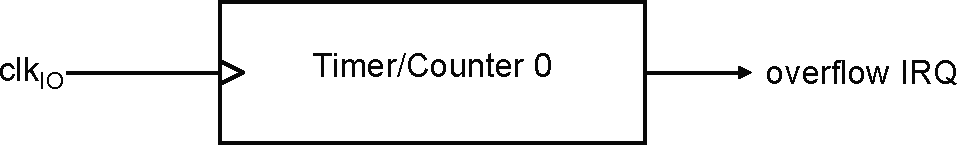
\includegraphics[scale=\figscale]{images/timsimpletc0}
\caption{Eenvoudige voorstelling van de Normal modus van Timer/Counter 0.}
\label{fig:timsimpletc0}
\end{figure}

%%%Zoals te zien is, kan in de Normal modus een interrupt gegenereerd worden als
%%%de waarde in het TCNT0-register van 255 naar 0 gaat (roll-over). Dit wordt
%%%de Timer Overflow interrupt genoemd.

Het TCNT0-register is door de gebruiker te lezen en te schrijven. Als de
software een waarde schrijft in TCNT0, dan gaat T/C0 verder tellen vanaf
deze waarde. Het is dan eenvoudig om te bepalen of de teller een bepaalde
waarde heeft. In listing~\ref{cod:waittc0} is te zien hoe TCNT0 eerst
geladen wordt met 0 en dan gewacht wordt totdat TCNT0 de waarde~123 heeft
bereikt.

\begin{figure}[!ht]
\begin{lstlisting}[language=AVRassembler,caption=Lezen van de tellerwaarde van T/C0.,label=cod:waittc0]
       ldi  r16,0        ; load TCNT0 with 0
       out  TCNT0,r16

wait:  in   r16,TCNT0    ; wait for TCNT0 to reach 123
       cpi  r16,123
       brne wait
\end{lstlisting}
\end{figure}

\subsection{Clear Timer on Compare Match Mode (CTC)}
\label{sec:tc0ctcmode}
In deze modus telt T/C0 vanaf 0 tot en met een opgegeven maximum en begint
dan weer op 0. Het opgegeven maximum wordt aangegeven door het Output Compare
Register (OCR0). Dit register moet voor aanvang van het tellen door de
gebruiker geladen worden met een waarde. Het is mogelijk om op een
\textsl{compare match} een interrupt te genereren. Een eenvoudige
voorstelling van de CTC-modus is te zien in figuur~\ref{fig:timsimplectctc0}.

\begin{figure}[!ht]
\centering
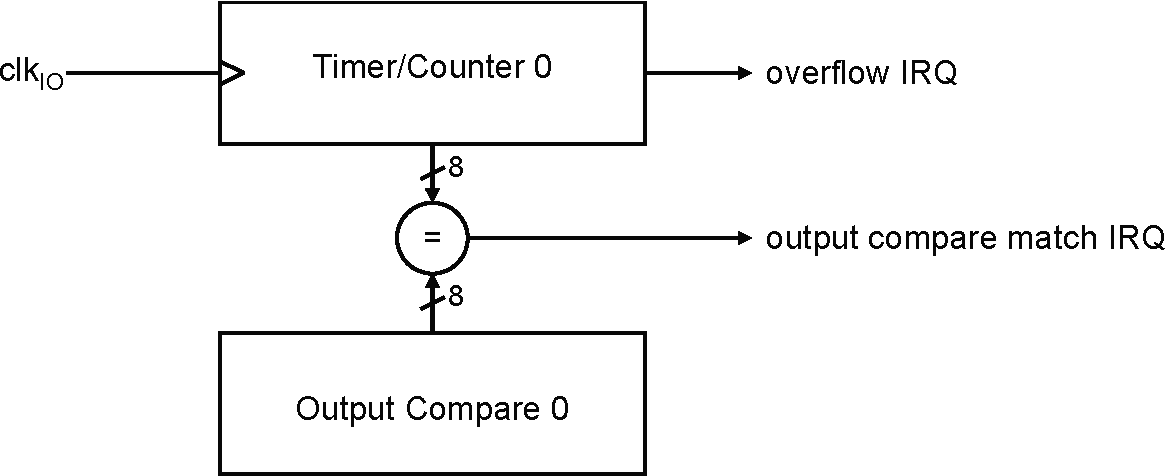
\includegraphics[scale=\figscale]{images/timsimplectctc0}
\caption{Eenvoudige voorstelling van de CTC-modus van Timer/Counter 0.}
\label{fig:timsimplectctc0}
\end{figure}

Zoals te zien is, kan in de CTC-modus een interrupt gegenereerd worden als
de waarde in het TCNT0-register en OCR0-register gelijk zijn. Dit wordt
de Output Compare Match interrupt genoemd. Merk op dat de interrupt pas
gegenereerd wordt als TCNT0 weer op~0 staat.

In listing~\ref{cod:setupocr0tc0} is te zien hoe het OCR0-register wordt
ingesteld op de waarde 143. Tevens wordt de CTC-modus geselecteerd in het
TCCR0-register. Merk op dat de teller na 144 klokpulsen weer op 0 staat.
De teller telt immers van 0 t/m 143.

\begin{figure}[!ht]
\begin{lstlisting}[language=AVRassembler,caption=Instellen van het OCR0-register van T/C0,label=cod:setupocr0tc0]
       ldi  r16,143          ; load OCR0 with 143
       out  OCR0,r16
       
       ldi  r16,0b00001000   ; select CTC mode 
       out  TCCR0,r16
\end{lstlisting}
\end{figure}

\subsection{Klokbronnen}
Al eerder is aangegeven dat T/C0 kan tellen op een intern kloksignaal of
op een extern kloksignaal. Aangezien de interne klokfrequentie vrij groot is
en het aantal timer-bits klein, zal T/C0 zeer snel op het maximum zitten en
genereert zodanig heel vaak een \textsl{timer overflow}. Vaak willen we de
timer overflow op een veel lagere frequentie laten plaatsvinden.
Een \textsl{prescaler} biedt dan uitkomst. Een prescaler is een digitale
schakeling die het aangeboden kloksignaal `deelt' door een getal, meestal een
macht van 2. Hierdoor telt T/C0 op een (veel) lagere frequentie. De prescaler
van T/C0 heeft vier mogelijke delers: 8, 64, 256 en 1024. Staat de prescaler
bijvoorbeeld op 1024 ingesteld dan wordt TCNT0 om de 1024 klokpulsen met
\'e\'en verhoogd. Dat betekent dat er eens in de~1024$\times$256 = 262144
klokpulsen 
een roll-over plaatsvindt.

Naast interne klokpulsen kan T/C0 ook externe klokpulsen tellen. Eigenlijk
telt TC/0 op \textsl{flanken}. Zo kan T/C0 op opgaande of neergaande flanken
tellen. Het externe kloksignaal moet worden aangeboden aan ingang T0
(pin 1 op een 40-pin PDIP). De prescaler kan niet ingeschakeld worden bij
gebruik van externe klokpulsen.

Natuurlijk kan T/C0 ook ``uit'' staan. T/C0 is dan gestopt met tellen. Dit is
de situatie direct na een reset.
Bij elkaar levert dit acht mogelijke klokbronnen op. Ook ``uit'' noemen we een
klokbron en de teller kan ook direct met de systeemklok gevoed worden. Dit
is met drie bits aan te geven. Dit zijn de CS0-bits in register TCCR0.

In figuur~\ref{fig:timsimplenormalctctc0} is een vereenvoudigde weergave
te zien van T/C0 met de klokbronselectie en normal- en CTC-modi. In
figuur~\ref{fig:timtccr0csbits} is de indeling van de CS0-bits in het
TCCR0-register te zien. De betekenis van de CS0-bits is te vinden in
tabel~\ref{tab:timklokselectie0}.

\begin{figure}[!ht]
\centering
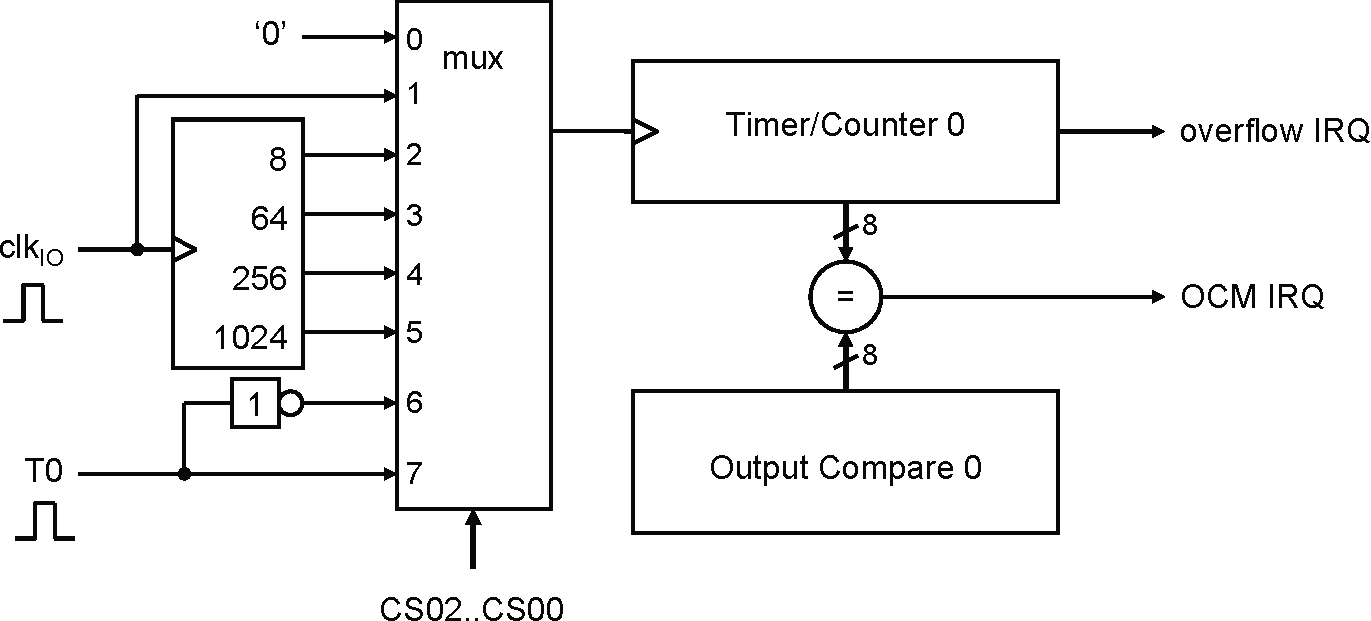
\includegraphics[scale=\figscale]{images/timsimplenormalctctc0}
\caption{Eenvoudige voorstelling van de normal en CTC-modus van Timer/Counter 0.}
\label{fig:timsimplenormalctctc0}
\end{figure}

%%%% TCCR0
\begin{registerdef}{De CS02-, CS01 en CS00-bits in het TCCR0-register}{fig:timtccr0csbits}
7 & 6 & 5 & 4 & 3 & 2 & 1 & 0 \\
\hline
\multicolumn{1}{|c}{\cellcolor{regcell} FOC0} & \multicolumn{1}{|c}{\cellcolor{regcell}WGM00} & \multicolumn{1}{|c}{\cellcolor{regcell} COM01} & \multicolumn{1}{|c}{\cellcolor{regcell} COM00} & \multicolumn{1}{|c}{\cellcolor{regcell} WGM01} & \multicolumn{1}{|c}{CS02} & \multicolumn{1}{|c}{CS01} & \multicolumn{1}{|c|}{CS00} \\ \hline
W & R/W & R/W & R/W & R/W & R/W & R/W & R/W \\
0 & 0 & 0 & 0 & 0 & 0 & 0 & 0 \\
\end{registerdef}
%%%% TCCR0

\begin{table}[!ht]
\centering
\caption{Klokbronselectie voor Timer/Counter 0.}
\label{tab:timklokselectie0}
\renewcommand\arraystretch{1.2}
%\tabulinesep=1.2mm
\begin{tabu} to 0.5\textwidth{ccc|l}
CS02 & CS01 & CS00 & operatie \\ \hline
  0  &   0  &   0  & geen werking, klok is gestopt\\
  0  &   0  &   1  & $\text{CLK}_\text{IO}/1$, geen prescaler \\
  0  &   1  &   0  & $\text{CLK}_\text{IO}/8$, van prescaler \\ 
  0  &   1  &   1  & $\text{CLK}_\text{IO}/64$, van prescaler \\
  1  &   0  &   0  & $\text{CLK}_\text{IO}/256$, van prescaler \\
  1  &   0  &   1  & $\text{CLK}_\text{IO}/1024$, van prescaler \\
  1  &   1  &   0  & externe klokbron op de T0-pin, neergaande flank \\
  1  &   1  &   1  & externe klokbron op de T0-pin, opgaande flank \\
\end{tabu}
\end{table}

De code in listing~\ref{cod:setupctcprescaler1024tc0} zorgt ervoor dat T/C0
ingesteld wordt in CTC-modus met een prescalerwaarde van 1024 als klokbron.

\begin{figure}[!ht]
\begin{lstlisting}[language=AVRassembler,caption=Selectie van CTC-modus en prescaler 1024.,label=cod:setupctcprescaler1024tc0]
       ldi  r16,0b00001101   ; select CTC mode, prescaler 1024
       out  TCCR0,r16
\end{lstlisting}
\end{figure}

\subsection{Interrupts: Timer overflow en Output Compare Match overflow}
Een taak die vaak voorkomt in de ATmega32, is het periodiek uitvoeren
van een stukje code. Te denken valt aan een temperatuurmeting die elke
minuut moet plaatsvinden. Natuurlijk kunnen we een wachtlus gebruiken,
maar de controller kan dan niets anders doen. We kunnen T/C0 gebruiken
om een stukje tijd af te meten.

In de normal-modus telt T/C0 van 0 t/m 255.
Als T/C0 een roll-over heeft, dus van telstand 255 naar telstand 0 gaat,
wordt op telstand~0 de Timer/Counter 0 Overflow Flag (TOV0) op~1 gezet.
In figuur~\ref{fig:tc0tov0} is dit grafisch uitgebeeld. Elke keer als
de teller weer op 0 staat, wordt de TOV-vlag op 1 gezet. De TOV0-vlag is
terug te vinden in het Timer/Counter Interrupt Flag Register (TIFR).

\begin{figure}[!ht]
\centering
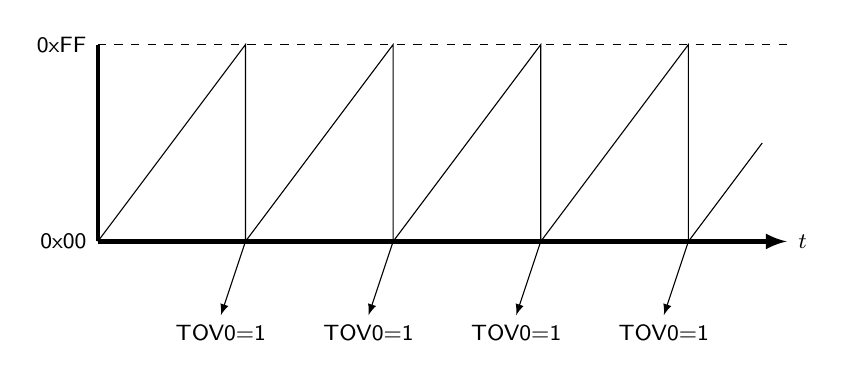
\begin{tikzpicture}[font=\footnotesize\sffamily,>=latex,scale=1.25]
\coordinate (A) at (0,0);
\draw [ultra thick] (A) node[left] {0x00} -- ++(0,2) node[left] {0xFF};
\draw (A) -- ++(1.5,2) -- ++(0,-2) -- ++(1.5,2) -- ++(0,-2) -- ++(1.5,2) -- ++(0,-2) -- ++(1.5,2) -- ++(0,-2) -- ++(0.75,1);
\draw [ultra thick,->](A) -- (7,0) node[right] {$t$};
\draw [dashed] (0,2) -- (7,2) {};
\draw [->] (1.5,0) -- ++(-0.25,-0.75) node[below] {TOV0=1};
\draw [->] (3.0,0) -- ++(-0.25,-0.75) node[below] {TOV0=1};
\draw [->] (4.5,0) -- ++(-0.25,-0.75) node[below] {TOV0=1};
\draw [->] (6.0,0) -- ++(-0.25,-0.75) node[below] {TOV0=1};
\end{tikzpicture}
\caption{Tijddiagram van de TCNT0-waarde met de momenten van een timer overflow.}
\label{fig:tc0tov0}
\end{figure}

De TOV0-vlag is op twee manieren op 0 te krijgen: door hardware bij het
uitvoeren van een timer overflow interrupt en door software door het
schrijven van een 1 in het TIFR-register. De frequentie van de timer overflow
is te berekenen met de formule:
%
\begin{equation}
f_{ov} = \dfrac{f_{clk}}{\mathrm{prescaler}\times 256}
\end{equation}
%
Bij een frequentie van 3,6864 MHz en een prescalerwaarde van 1024 is de
overflow-frequentie dus 14,0625 Hz. Merk op dat bij deze klokfrequentie
de overflow-frequentie niet lager te realiseren is.

%%%% TIFR
\begin{registerdef}{Het TIFR-register}{fig:tc0tifr}
7 & 6 & 5 & 4 & 3 & 2 & 1 & 0 \\
\hline
\multicolumn{1}{|c}{\cellcolor{regcell} OCF2} & \multicolumn{1}{|c}{\cellcolor{regcell} TOV2} & \multicolumn{1}{|c}{\cellcolor{regcell} ICF1} & \multicolumn{1}{|c}{\cellcolor{regcell} OCF1A} & \multicolumn{1}{|c}{\cellcolor{regcell} OCF1B} & \multicolumn{1}{|c}{\cellcolor{regcell} TOV1} & \multicolumn{1}{|c}{OCF0} & \multicolumn{1}{|c|}{TOV0} \\ \hline
R/W & R/W & R/W & R/W & R/W & R/W & R/W & R/W \\
0 & 0 & 0 & 0 & 0 & 0 & 0 & 0 \\
\end{registerdef}
%%%% TIFR

\begin{figure}[!ht]
\centering
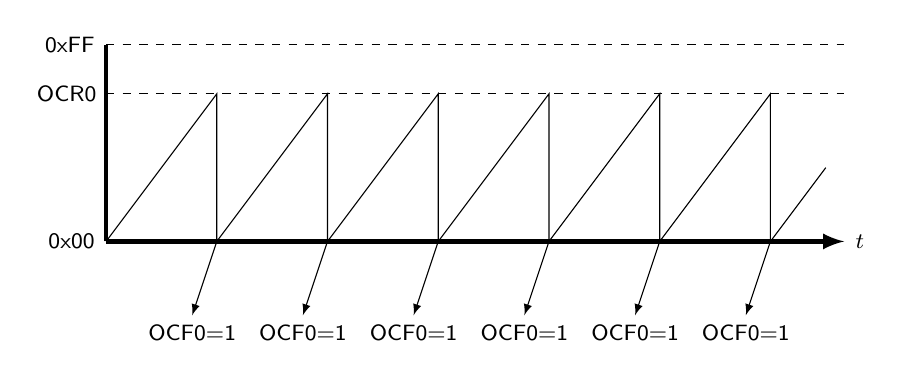
\begin{tikzpicture}[font=\footnotesize\sffamily,>=latex,scale=1.25]
\coordinate (A) at (0,0);
\draw [ultra thick] (A) node[left] {0x00} -- ++(0,2) node[left] {0xFF};
\draw (A) -- ++(1.125,1.5) -- ++(0,-1.5) -- ++(1.125,1.5) -- ++(0,-1.5) -- ++(1.125,1.5) -- ++(0,-1.5) -- ++(1.125,1.5) -- ++(0,-1.5) -- ++(1.125,1.5) -- ++(0,-1.5) -- ++(1.125,1.5) -- ++(0,-1.5) -- ++(0.5625,0.75);
\draw [ultra thick,->](A) -- (7.5,0) node[right] {$t$};
\draw [dashed] (0,2) -- (7.5,2) {};
\draw (0,1.5) node[left] {OCR0};
\draw [dashed] (0,1.5) -- (7.5,1.5) {};
\draw [->] (1.125,0) -- ++(-0.25,-0.75) node[below] {OCF0=1};
\draw [->] (2.250,0) -- ++(-0.25,-0.75) node[below] {OCF0=1};
\draw [->] (3.375,0) -- ++(-0.25,-0.75) node[below] {OCF0=1};
\draw [->] (4.500,0) -- ++(-0.25,-0.75) node[below] {OCF0=1};
\draw [->] (5.625,0) -- ++(-0.25,-0.75) node[below] {OCF0=1};
\draw [->] (6.750,0) -- ++(-0.25,-0.75) node[below] {OCF0=1};
\end{tikzpicture}
\captionsetup{width=.85\linewidth}
\caption{Tijddiagram van de TCNT0-waarde met de momenten van een output compare match overflow.}
\label{fig:}
\end{figure}














\subsection{Fast-PWM mode}
\label{sec:tc0fastpwmmode}
Volgt nog.

\subsection{Phase Correct PWM mode}
\label{sec:tc0phasecorrectpwmmode}
Volgt nog.







\section{De registers van Timer/Counter 0}
De besturing van Timer/Counter 0 is vastgelegd in het TCCR0-register, zie
figuur~\ref{fig:tccr0}. Dit register kan zowel gelezen als geschreven worden.

%%%% TCCR0
\begin{registerdef}{TCCR0 register}{fig:tccr0}
7 & 6 & 5 & 4 & 3 & 2 & 1 & 0 \\
\hline
\multicolumn{1}{|c}{FOC0} & \multicolumn{1}{|c}{WGM00} & \multicolumn{1}{|c}{COM01} & \multicolumn{1}{|c}{COM00} & \multicolumn{1}{|c}{WGM01} & \multicolumn{1}{|c}{CS02} & \multicolumn{1}{|c}{CS01} & \multicolumn{1}{|c|}{CS00} \\ \hline
W & R/W & R/W & R/W & R/W & R/W & R/W & R/W \\
0 & 0 & 0 & 0 & 0 & 0 & 0 & 0 \\
\end{registerdef}
%%%% TCCR0

\textbf{Bit 7 -- FOC0: Force Output Compare}\\
De FOC0-bit is alleen actief als we de WGM0\textsl{x}-bits non-PWM-modus specificeren. Bij
het specificeren van \'e\'en van de twee PWM-modi moet deze bit altijd als 0 geschreven
worden. Als deze bit met een 1 geladen wordt, zal de signaalvormgenerator een directe
compare match krijgen en zal de OC0-uitgang veranderen zoals is vastgelegd in de
COM0\textsl{x}-bits.

%%%The FOC0 bit is only active when the WGM00 bit specifies a non-PWM mode. However, for
%%%ensuring compatibility with future devices, this bit must be set to zero when TCCR0 is written
%%%when operating in PWM mode. When writing a logical one to the FOC0 bit, an immediate compare
%%%match is forced on the Waveform Generation unit. The OC0 output is changed according to
%%%its COM01:0 bits setting. Note that the FOC0 bit is implemented as a strobe. Therefore it is the
%%%value present in the COM01:0 bits that determines the effect of the forced compare.

\textbf{Bits 3,6 -- WGM0\textsl{x} signaalvormgeneratorbits}\\
Deze bits bepalen de telvolgorde van de Timer/Counter, de maximale telwaarde en het type
van de signaalvormgenerator. Zie tabel~\ref{tab:signaalvormgeneratie0}.

\begin{table}[!ht]
\centering
\caption{Signaalvormgeneratie}
\label{tab:signaalvormgeneratie0}
\renewcommand\arraystretch{1.2}
\begin{tabu} {cc|l|l|l|l}
WGM01 & WGM00 & Modus & Top & Update OCR0 & TOV0-vlag \\ \hline
  0   &   0   & Normaal & 255 & direct & 255 \\
  0   &   1   & Phase Correct PWM & 255 & 255 & 0 \\
  1   &   0   & CTC & OCR0 & direct & 255 \\
  1   &   1   & Fast PWM & 255 & 0 & 255
\end{tabu}
\end{table}

\textbf{Bits 5,4 -- COM0\textsl{x} Compare Match Output Mode}\\
Deze bits bepalen het gedrag van de Output Compare pin (OC0).
Merk op dat de Data Direction (DDR) bit van de OC0-pin op 1 gezet
moet worden om de uitgang te activeren.
Tabel~\ref{tab:comparematchnonpwm0} geeft de functionaliteit van
de COM0\textsl{x}-bits weer in non-PWM-modus (Normal en CTC).

\begin{table}[!ht]
\centering
\caption{Compare Match uitgang, non-PWM-modus.}
\label{tab:comparematchnonpwm0}
\renewcommand\arraystretch{1.2}
\begin{tabu} {cc|l}
COM01 & COM00 & Beschrijving \\ \hline
  0   &   0   & Normale poortwerking, OC0 is gedeactiveerd \\
  0   &   1   & Verander OC0 op een compare match (toggle) \\
  1   &   0   & Zet OC0 op 0 op een compare match \\
  1   &   1   & Zet OC0 op 1 op een compare match \\
\end{tabu}
\end{table}

Tabel~\ref{tab:comparematchfastpwm0} geeft de functionaliteit van de
COM0\textsl{x}-bits weer in Fast PWM-modus.

\begin{table}[!ht]
\centering
\caption{Compare Match uitgang, Fast PWM-modus.}
\label{tab:comparematchfastpwm0}
\renewcommand\arraystretch{1.2}
\begin{tabu} {cc|l}
COM01 & COM00 & Beschrijving \\ \hline
  0   &   0   & Normale poortwerking, OC0 is gedeactiveerd \\
  0   &   1   & Niet gebruikt \\
  1   &   0   & Zet OC0 op 0 op een compare match, zet op 1 op TCNT = 255 \\
  1   &   1   & Zet OC0 op 1 op een compare match, zet op 0 op TCNT = 255 \\
\end{tabu}
\end{table}

Tabel~\ref{tab:comparematchphasecorrectpwm0} geeft de functionaliteit van de
COM0\textsl{x}-bits weer in Phase Correct PWM-modus.

\begin{table}[!ht]
\centering
\caption{Compare Match uitgang, Fast PWM-modus.}
\label{tab:comparematchphasecorrectpwm0}
\renewcommand\arraystretch{1.2}
\begin{tabu} {cc|p{11cm}}
COM01 & COM00 & Beschrijving \\ \hline
  0   &   0   & Normale poortwerking, OC0 is gedeactiveerd \\
  0   &   1   & Niet gebruikt \\
  1   &   0   & Zet OC0 op 0 bij Compare Match bij omhoog tellen, zet OC0 op 1 bij omlaag tellen \\
  1   &   1   & Zet OC0 op 1 bij Compare Match bij omhoog tellen, zet OC0 op 0 bij omlaag tellen \\
\end{tabu}
\end{table}





\textbf{Bits 2,1,0 -- CS0\textsl{x} klokselectiebits}\\
In tabel~\ref{tab:klokselectie0} is te zien hoe een klok geselecteerd kan worden.

\begin{table}[!ht]
\centering
\caption{Klokselectie voor Timer/Counter 0.}
\label{tab:klokselectie0}
\renewcommand\arraystretch{1.2}
%\tabulinesep=1.2mm
\begin{tabu} to 0.5\textwidth{ccc|l}
CS02 & CS01 & CS00 & operatie \\ \hline
  0  &   0  &   0  & geen werking, klok is gestopt\\
  0  &   0  &   1  & $\text{CLK}_\text{IO}/1$, geen prescaler \\
  0  &   1  &   0  & $\text{CLK}_\text{IO}/8$, van prescaler \\ 
  0  &   1  &   1  & $\text{CLK}_\text{IO}/64$, van prescaler \\
  1  &   0  &   0  & $\text{CLK}_\text{IO}/256$, van prescaler \\
  1  &   0  &   1  & $\text{CLK}_\text{IO}/1024$, van prescaler \\
  1  &   1  &   0  & externe klokbron op de T0-pin, neergaande flank \\
  1  &   1  &   1  & externe klokbron op de T0-pin, opgaande flank \\
\end{tabu}
\end{table}


Het TCNT0-register is een 8-bits register en bevat de tellerwaarde van Timer/Counter~0,
zie figuur~\ref{fig:tcnt0}. Dit register kan zowel gelezen als geschreven worden. Bij
een schrijfactie telt Timer/Counter~0 verder vanaf de geschreven waarde.

%%%% TCNT0
\begin{registerdef}{Het TCNT0 register}{fig:tcnt0}
7 & 6 & 5 & 4 & 3 & 2 & 1 & 0 \\
\hline
\multicolumn{8}{|c|}{TCNT0[7:0]}  \\ \hline
R/W & R/W & R/W & R/W & R/W & R/W & R/W & R/W \\
0 & 0 & 0 & 0 & 0 & 0 & 0 & 0 \\
\end{registerdef}
%%%% TCNT0

Het OCR0-register bevat een 8-bits waarde en wordt continue vergeleken met de waarde
in het TCNT0-register, zie figuur~\ref{fig:ocr0}. Als de twee register gelijk zijn aan
elkaar kan een interrupt gegenereerd worden of kan een golfvorm gegenereerd worden op
de OC0-uitgang.

%%%% OCR0
\begin{registerdef}{Het OCR0 register}{fig:ocr0}
7 & 6 & 5 & 4 & 3 & 2 & 1 & 0 \\
\hline
\multicolumn{8}{|c|}{OCR0[7:0]}  \\ \hline
R/W & R/W & R/W & R/W & R/W & R/W & R/W & R/W \\
0 & 0 & 0 & 0 & 0 & 0 & 0 & 0 \\
\end{registerdef}
%%%% OCR0








De indeling van het TIMSK-register is te zien in figuur~\ref{fig:timsk}. Voor Timer/Counter~0
zijn alleen de bits OCIE0 (bit 1) en TOIE0 (bit 0) van belang.

%%%% TIMSK
\begin{registerdef}{Het TIMSK register}{fig:timsk}
7 & 6 & 5 & 4 & 3 & 2 & 1 & 0 \\
\hline
\multicolumn{1}{|c}{\cellcolor{regcell} OCIE2} & \multicolumn{1}{|c}{\cellcolor{regcell} TOIE2} & \multicolumn{1}{|c}{\cellcolor{regcell} TICIE1} & \multicolumn{1}{|c}{\cellcolor{regcell} OCIE1A} & \multicolumn{1}{|c}{\cellcolor{regcell} OCIE1B} & \multicolumn{1}{|c}{\cellcolor{regcell} TOIE1} & \multicolumn{1}{|c}{OCIE0} & \multicolumn{1}{|c|}{TOIE0} \\ \hline
R/W & R/W & R/W & R/W & R/W & R/W & R/W & R/W \\
0 & 0 & 0 & 0 & 0 & 0 & 0 & 0 \\
\end{registerdef}
%%%% TIMSK

\textbf{Bit 1 -- OCIE0: Timer/Counter 0 Output Compare Match Interrupt Enable} \\
Een logische 1 in deze bit zorgt ervoor dat de compare match interrupt geactiveerd wordt.
Een interrupt wordt pas daadwerkelijk uitgevoerd als de I-bit in het statusregister ook
een logische 1 is.

\textbf{Bit 0 -- TOIE0: Timer/Counter 0 Overflow Interrupt Enable} \\
Een logische 1 in deze bit zorgt ervoor dat de overflow interrupt geactiveerd wordt.
Een interrupt wordt pas daadwerkelijk uitgevoerd als de I-bit in het statusregister ook
een logische 1 is.

De indeling van het TIFR-register is te zien in figuur~\ref{fig:tifr}. Voor Timer/Counter~0
zijn alleen de bits OCF0 (bit 1) en TOV0 (bit 0) van belang.

%%%% TIFR
\begin{registerdef}{Het TIFR register}{fig:tifr}
7 & 6 & 5 & 4 & 3 & 2 & 1 & 0 \\
\hline
\multicolumn{1}{|c}{\cellcolor{regcell} OCF2} & \multicolumn{1}{|c}{\cellcolor{regcell} TOV2} & \multicolumn{1}{|c}{\cellcolor{regcell} ICF1} & \multicolumn{1}{|c}{\cellcolor{regcell} OCF1A} & \multicolumn{1}{|c}{\cellcolor{regcell} OCF1B} & \multicolumn{1}{|c}{\cellcolor{regcell} TOV1} & \multicolumn{1}{|c}{OCF0} & \multicolumn{1}{|c|}{TOV0} \\ \hline
R/W & R/W & R/W & R/W & R/W & R/W & R/W & R/W \\
0 & 0 & 0 & 0 & 0 & 0 & 0 & 0 \\
\end{registerdef}
%%%% TIFR

\textbf{Bit 1 -- OCF0: Output Compare Flag 0} \\
Deze bit wordt op een logische 1 gezet als de waarde van het OCR0-register gelijk is aan
de waarde in het TCNT0-register (compare match). Dit gebeurt op de volgende Timer/Counter
0 klokpuls. Deze bit wordt op een logische~0 gezet
als de bijbehorende interrupt wordt uitgevoerd. Als alternatief voor het op 0 zetten
kan een 1 worden geschreven naar deze bit.

\textbf{Bit 0 -- TOV0: Timer/Counter 0 Overflow Flag} \\
Deze bit wordt op een logische 1 gezet als Timer/Counter 0 een overflow veroorzaakt. Dit
gebeurt op de volgende Timer/Counter 0 klokpuls. Deze
bit wordt op 0 gezet als de bijbehorende interrupt wordt uitgevoerd. Als alternatief voor
het op 0 zetten kan een 1 worden geschreven naar deze bit. In fasecorrect PWM-modus wordt
deze bit op 1 gezet als Timer/Counter 0 van telrichting verandert op 0.

In figuur~\ref{fig:intsfior} is het SFIOR-register te zien.

%%%% SFIOR
\begin{registerdef}{Het SFIOR register}{fig:intsfior}
7 & 6 & 5 & 4 & 3 & 2 & 1 & 0 \\
\hline
\multicolumn{1}{|c}{\cellcolor{regcell} ADTS2} & \multicolumn{1}{|c}{\cellcolor{regcell} ADTS1} & \multicolumn{1}{|c}{\cellcolor{regcell} ADTS0} & \multicolumn{1}{|c}{\cellcolor{regcell} --} & \multicolumn{1}{|c}{\cellcolor{regcell} ACME} & \multicolumn{1}{|c}{\cellcolor{regcell} PUD} & \multicolumn{1}{|c}{\cellcolor{regcell}PSR2} & \multicolumn{1}{|c|}{PRS10} \\ \hline
R/W & R/W & R/W & R & R/W & R/W & R/W & R/W \\
0 & 0 & 0 & 0 & 0 & 0 & 0 & 0 \\
\end{registerdef}
%%%% SFIOR

\textbf{Bit 0 -- PRS10: Prescaler reset Timer/Counter 1 en Timer/Counter 0}\\
Wanneer deze bit met een 1 geschreven wordt, zal de prescaler van Timer/Counter 1 en
Timer/Counter 0 worden gereset. Nadat de operatie is voltooid, wordt deze bit door de
hardware op 0 gezet. Merk op dat de prescaler door zowel Timer/Counter 1 als
Timer/Counter 0 gebruikt wordt. Het beïnvloedt de werking van beide Timer/Counters.
Deze bit leest altijd als een 0.

\endinput